%
% teil1.tex -- Beispiel-File für das Paper
%
% (c) 2020 Prof Dr Andreas Müller, Hochschule Rapperswil
%
% !TEX root = ../../buch.tex
% !TEX encoding = UTF-8
%
\section{Approximative geradlinige Bewegung
\label{geradlinig:section:approximative_geradlinig}}
\kopfrechts{Approximative geradlinige Bewegung}
Der erste approximative geradliniger Mechanismus war derjenige in
James Watts Dampfmaschine, den er 1784 patentieren liess.
Es handelt sich dabei um eine approximative gerade Linie,
weil sie nur auf einem beschränktem Bereich gerade ist.
Der Pfad der erzeugt wird durch Watts Mechanismus wird 
auch Watts Kurve bezeichnet und im Spezialfall 
von Abbildung~\ref{fig:lemniskate} handelt es sich 
um die Lemniskate von Bernoulli.

\begin{figure}[htbp]
    \centering
    \begin{minipage}{0.32\textwidth}
        \centering
        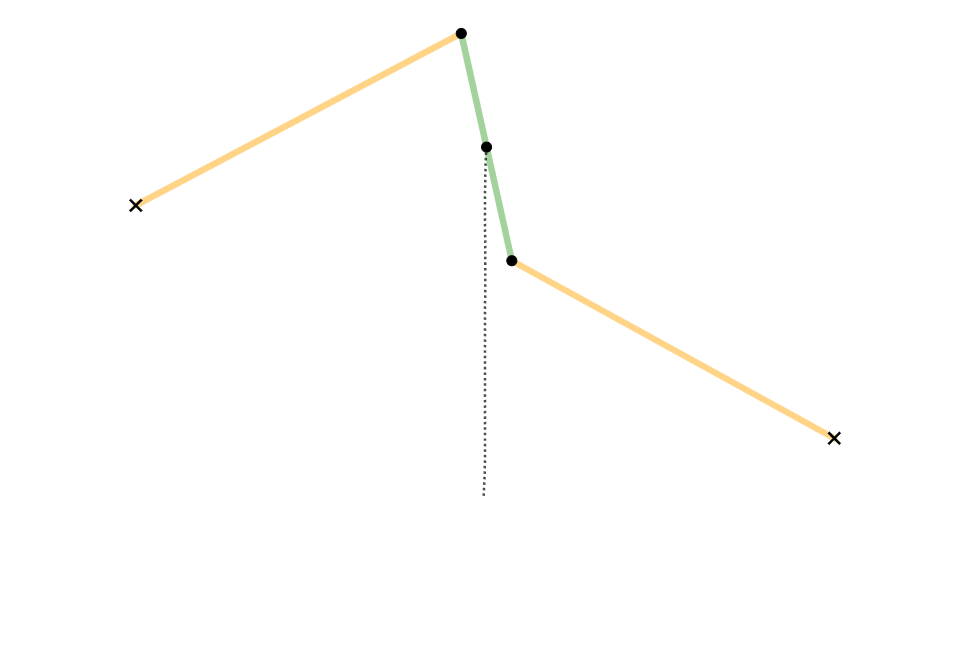
\includegraphics[width=\textwidth]{papers/geradlinig/figures/watts_linkage1.png}
    \end{minipage}
    \hfill
    \begin{minipage}{0.32\textwidth}
        \centering
        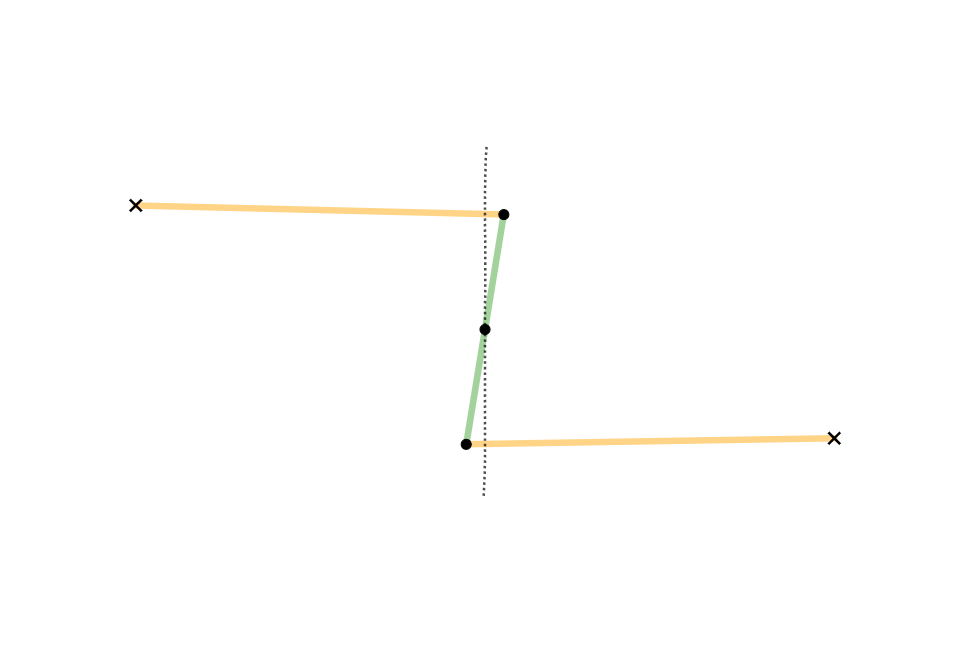
\includegraphics[width=\textwidth]{papers/geradlinig/figures/watts_linkage2.png}
    \end{minipage}
    \hfill
    \begin{minipage}{0.32\textwidth}
        \centering
        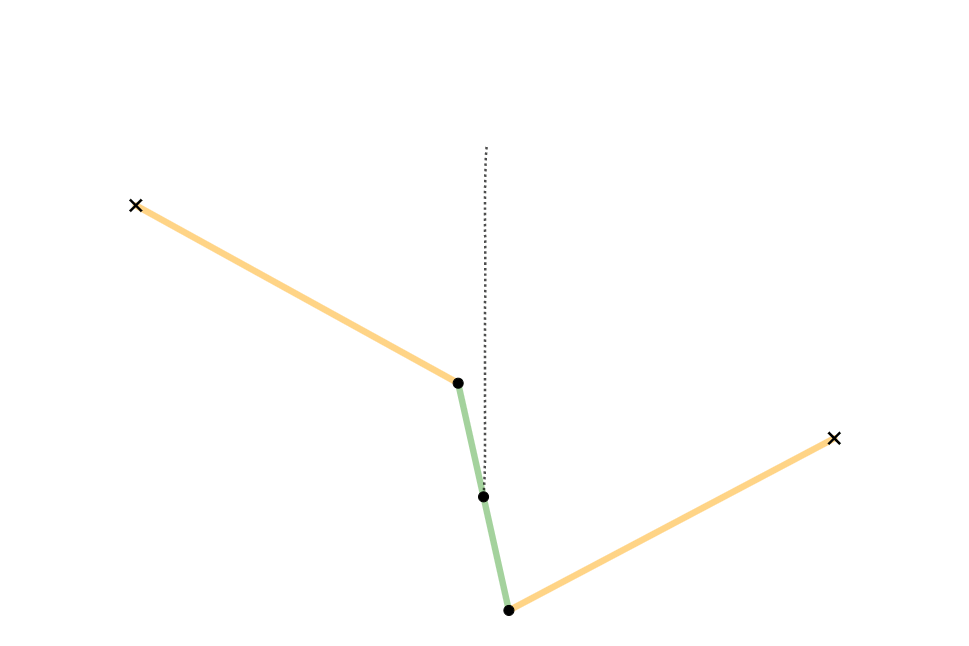
\includegraphics[width=\textwidth]{papers/geradlinig/figures/watts_linkage3.png}
    \end{minipage}
    \caption{Der Mechanismus von Watt~\cite{watt_linkage}.}
    \label{fig:watts_link}
\end{figure}

\begin{figure}[htbp]
    \centering
    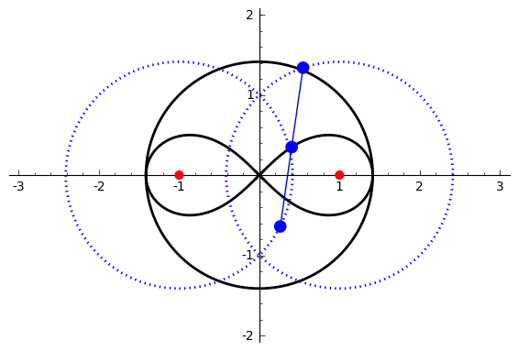
\includegraphics[width=0.5\textwidth]{papers/geradlinig/figures/lemniskate.png}
    \caption{Lemniskate von Bernoulli als Spezialfall der Wattskurve~\cite{watt_curve}.} 
~\label{fig:lemniskate}
\end{figure}

\begin{figure}[htbp]
    \centering
    \begin{minipage}{0.32\textwidth}
        \centering
        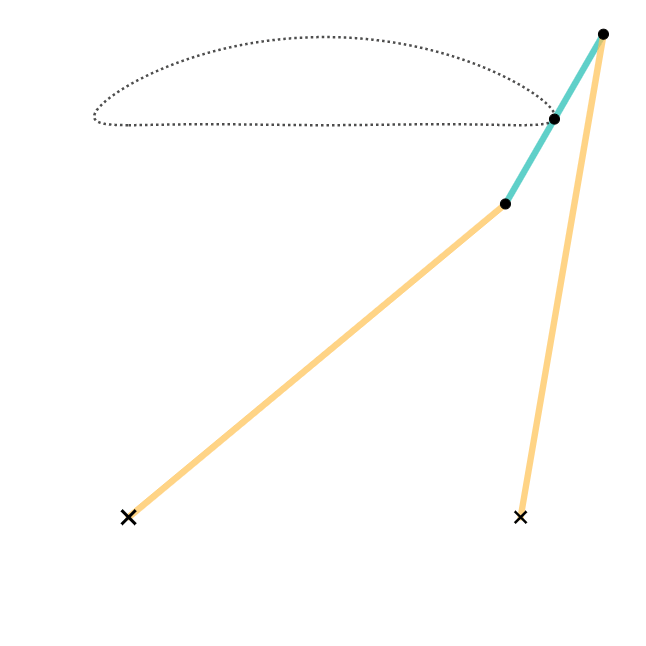
\includegraphics[width=\textwidth]{papers/geradlinig/figures/chebyshev_linkage1.png}
    \end{minipage}
    \hfill
    \begin{minipage}{0.32\textwidth}
        \centering
        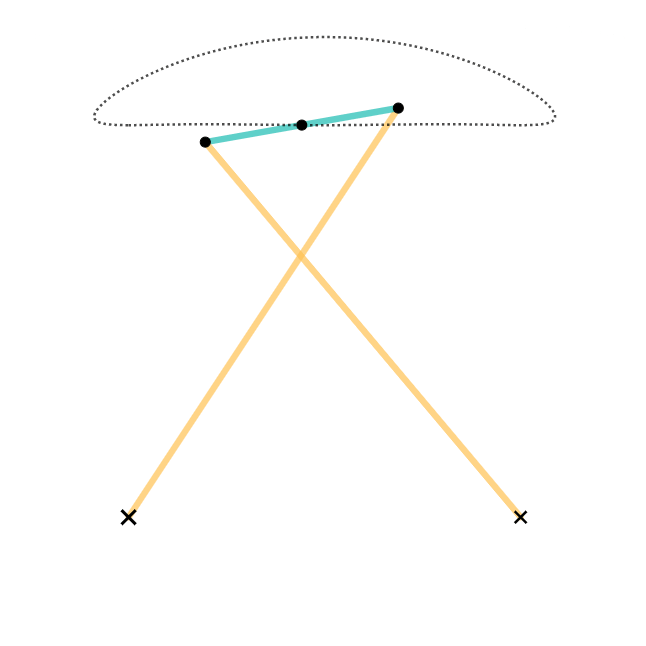
\includegraphics[width=\textwidth]{papers/geradlinig/figures/chebyshev_linkage2.png}
    \end{minipage}
    \hfill
    \begin{minipage}{0.32\textwidth}
        \centering
        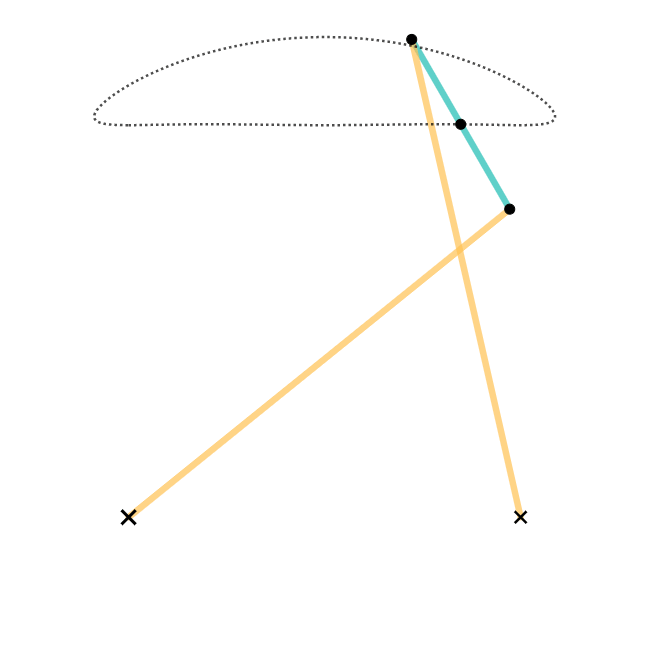
\includegraphics[width=\textwidth]{papers/geradlinig/figures/chebyshev_linkage3.png}
    \end{minipage}
    \caption{Der Mechanismus von Chebyshev~\cite{chebyshev_linkage}.}
    \label{fig:chebyshev_link}
\end{figure}


